\subsection{Ondas estacionárias de som: geração de harmônicos
em função da frequência f}

O segundo experimento consiste em analisar a geração de harmônicos em função da variação da frequência de ondas sonoras. Para isso, será utilizado um dispositivo conhecido como Tubo de Kundt para gerar ondas de som estacionárias que se propagam no ar com o comprimento da coluna L fixo, que pode ser representado na Imagem a seguir:

\begin{figure}[H]
  \centering
  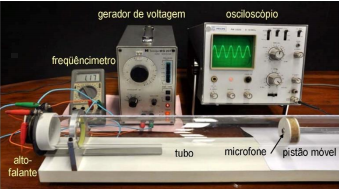
\includegraphics[scale=1.15]{images/Tubo de Kundt.png}
  \caption{ Esquema do dispositivo para a geração de ondas de som estacionárias no interior de um tubo cilíndrico.}
\end{figure}

O alto-falante presente em uma das extremidades do dispositivo é excitado através de um gerador de voltagem harmônico com uma frequência \textit{f}. No extremo oposto, o tubo está fechado com um pistão móvel acoplado a um microfone que será responsável por captar as ondas sonoras. O sinal elétrico fornecido pelo microfone, proporcional à amplitude da pressão, é monitorado por meio de um osciloscópio (medidor de voltagem em função do tempo). O dispositivo pode ser representado esquematicamente pela Figura a seguir:

\begin{figure}[H]
  \centering
  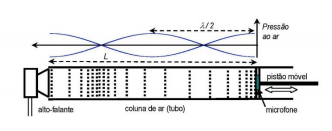
\includegraphics[scale=1.15]{images/esquemático tubo de Kundt.png}
  \caption{ Esquemático do experimento de geração de ondas de som estacionárias.}
\end{figure}

Inicialmente, desloca-se o pistão até um comprimento L fixo, preestabelecido, da coluna de ar. Posteriormente, varia-se a frequência do gerador de voltagem harmônica até que seja possível observar as ondas de pressão com a maior intensidade. Esse momento corresponde exatamente a geração de uma onda estacionária. Dessa relação, registra-se os valores \textit{$f_n$} correspondente aos sucessivos harmônicos.

\begin{figure}[H]
  \centering
  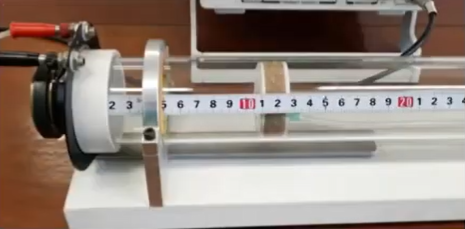
\includegraphics[scale=1.15]{images/comprimento L.png}
  \caption{ Registro do comprimento L fixado para o experimento.}
\end{figure}

Partindo desde o modo fundamental (n = 1), será construído uma tabela com os valores do índice n do harmônico e os valores das frequências $f_n$ correspondentes. Com esses dados, será feito um gráfico de $f_n$ em função de $n/2L$ para se registrar a relação observada e comparar com as equações que definem a onda estacionária para eventuais levantamentos.

Por fim, analisando os dados obtidos, aplica-se o método dos mínimos quadrados no gráfico construído para, então, determinar a velocidade das ondas de som no ar no experimento em questão. A partir desse dado e sabendo que a temperatura da sala é de 25 ºC,  será realizado uma comparação com valores de referência para concluir se o resultado é coerente com o experimento.